\section{Running Example}
\label{sec:granularityEx}
To see how different representations of the system requirements will alter the MIVC and minimal cut set computations, let us examine once again the simple sensor example system that was described in Chapter~\ref{chap:compFF}. In this simple AADL architecture, the environmental temperature and pressure is sent to a subsystem of sensors that contains a temp sensor and a pressure sensor, both of which receive the respective environmental inputs. If the temperature (or pressure) surpasses a given threshold, then the temp (pressure) sensor outputs a high indication. It also gives the temperature (pressure) reading seen at the sensor. A diagram showing two levels of the AADL implementation is shown in Figure~\ref{fig:sensorGran1}.  

\begin{figure}[h]
\begin{center}
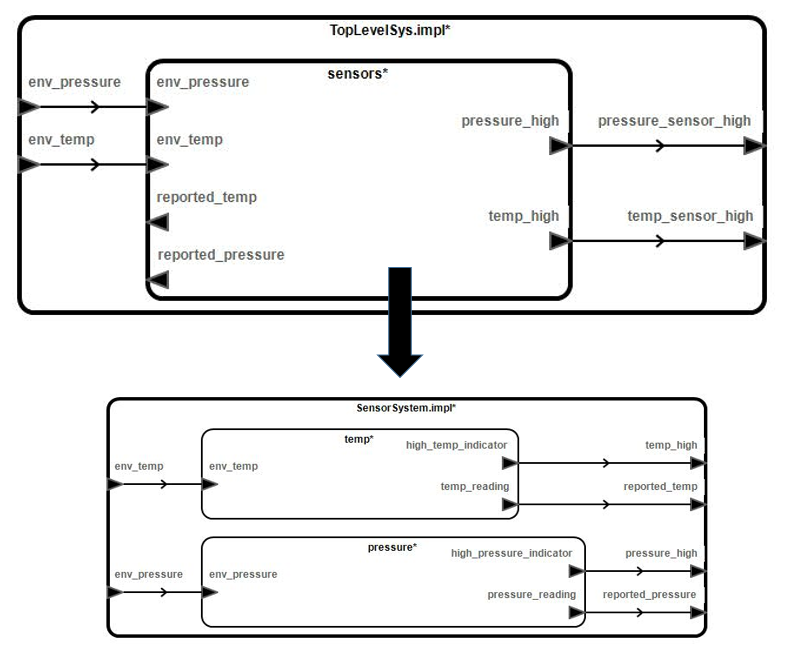
\includegraphics[width=14cm]{images/sensorGran.png}
\caption{Tempurature Sensor System} 
\label{fig:sensorGran1}
\end{center}
\end{figure}

Now that the basic architecture is in place, we focus our attention on the requirements of each component. The behavior we wish to enforce at the temperature sensor level corresponds to the following two guarantees, $G_1$ and $G_2$. (Note: the pressure sensor behavior is quite similar and for this reason, we will focus on the temperature for this example.) 

$G_1$: If the environmental temperature surpasses the threshold, $T_t$, then the system shall output a high temperature indication: \textit{(temp $> T_t$ ) $\implies$ (high\_temp\_indicator)}

$G_2$: The temperature read at the sensor is equivalent to the environmental temperature: \textit{temp = temp\_reading} 

These can be seen in the model as two distinct guarantees over the respective outputs of the sensor component. Assume that at the sensor, they are written exactly as above in two separate guarantees. Let us assume that system A is built by engineer A. The top level safety property states: 
\begin{center}
    \textit{If the environmental temperature reaches 90 degrees C, then the system shall report a high temperature indication.}
\end{center}

The direct subcomponent is the sensor system that contains the outputs: (1) a high temp indicator, and (2) the actual temperature. Engineer A chooses to write the supporting contract in the subsystem as follows: 
\begin{center}
    $g_A: (T_t \geq 90 \implies temp\_high) \land (temp\_indicator = T_t)$ 
\end{center}
The example temp sensor system contract hierarchy is shown in Figure~\ref{fig:granularityEx1}.  

\begin{figure}[h!]
\begin{center}
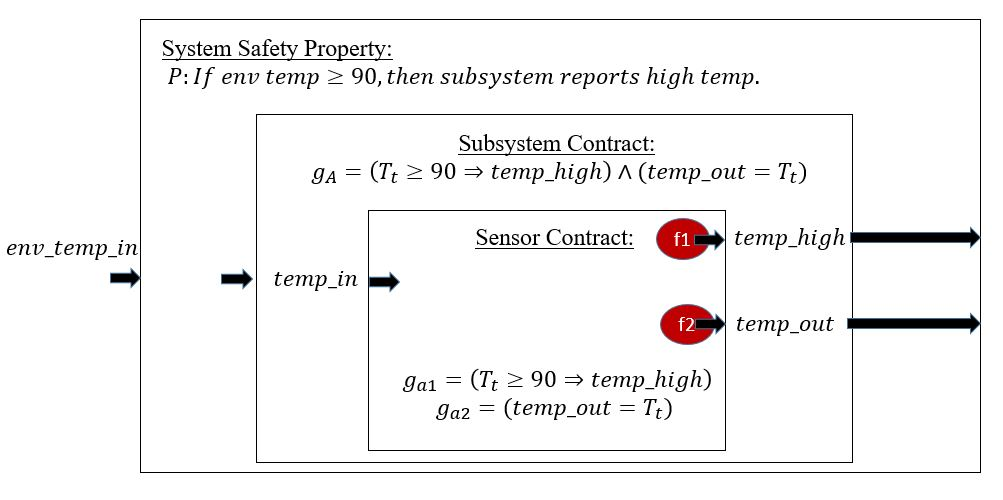
\includegraphics[width=10cm]{images/granEx1.jpg}
\caption{Temp Sensor System Contract Part I} \label{fig:granularityEx1}
\end{center}
\end{figure}

The safety property at the top level requires the contract $g_A$ for proof of validity. Thus, the \aivcalg will contain the contract $g_A$ as an MIVC. 

There are two faults defined for the temperature subsystem; one for each of the outputs. Fault $f_1$ affects the $temp\_high$ output and fault $f_2$ affects the $temp\_out$ output. Since each of these faults will violate the contract $g_A$, each of them will be found in the minimal cut set for $G_A$.

Now assume that Figure~\ref{fig:granularityEx2} was the system contract representation built by engineer B. 

\begin{figure}[h!]
\begin{center}
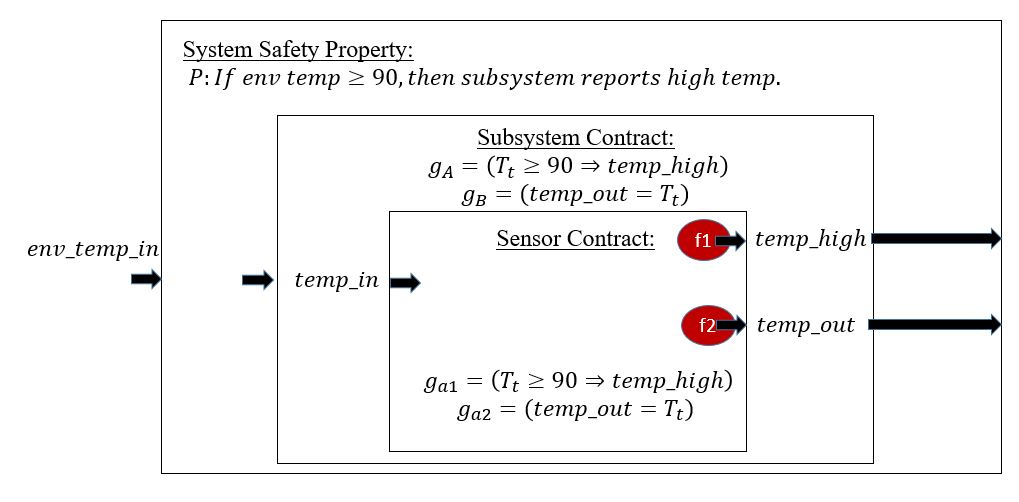
\includegraphics[width=10cm]{images/granEx2.jpg}
\caption{Temp Sensor System Contract Part II} \label{fig:granularityEx2}
\end{center}
\end{figure} 

The behavior and architecture of the system is the same, but the contract for the subsystem is more granular; it is stated as two separate contracts:
\begin{center}
    $ g_A = (T_t \geq 90 \implies temp\_high)$ \\ 
    $ g_B = (temp\_indicator = T_t)$ 
\end{center}

Since $g_B$ is not required for the proof of either the system safety property nor the subsystem level property, only $g_A$ is found in the MIVCs and thus only $f_1$ will be seen in the minimal cut set for this particular contract. 
 
In this example, it is easy to see how the granularity of the contracts may affect the results of analysis. Structurally (syntactically), the contracts written by engineer A and engineer B vary; yet logically they are equivalent. The proof of the nominal system holds in both cases. Yet, based on the architecture of the model and the formalization of the contracts, analysis results may be different. 

In the remainder of this chapter, we explore this problem through automation of contractual refinement and comparison of analysis results for both inductive validity cores and minimal cut sets. 